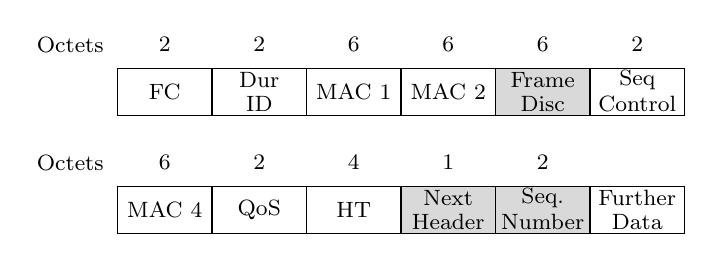
\begin{tikzpicture}[scale=0.6]
	\draw (0,0) rectangle (2,1);
	\draw (2,0) rectangle (4,1);
	\draw (4,0) rectangle (6,1);
	\draw (6,0) rectangle (8,1);
	\draw[fill=gray!30] (8,0) rectangle (10,1);
	\draw (10,0) rectangle (12,1);

	\draw (0,-1.5) rectangle (2,-2.5);
	\draw (2,-1.5) rectangle (4,-2.5);
	\draw (4,-1.5) rectangle (6,-2.5);
	\draw[fill=gray!30] (6,-1.5) rectangle (8,-2.5);
	\draw[fill=gray!30] (8,-1.5) rectangle (10,-2.5);
	\draw (10,-1.5) rectangle (12,-2.5);

	% Bits
	\draw (-1,1.5) node {\footnotesize Octets};
	\draw (1,1.5) node {\footnotesize 2};
	\draw (3,1.5) node {\footnotesize 2};
	\draw (5,1.5) node {\footnotesize 6};
	\draw (7,1.5) node {\footnotesize 6};
	\draw (9,1.5) node {\footnotesize 6};
	\draw (11,1.5) node {\footnotesize 2};

	\draw (-1,-1) node {\footnotesize Octets};
	\draw (1,-1) node {\footnotesize 6};
	\draw (3,-1) node {\footnotesize 2};
	\draw (5,-1) node {\footnotesize 4};
	\draw (7,-1) node {\footnotesize 1};
	\draw (9,-1) node {\footnotesize 2};
	

	% Fields
	\draw (1,0.5) node {\footnotesize FC};
	\draw (3,0.75) node {\footnotesize Dur};
	\draw (3,0.25) node {\footnotesize ID};
	\draw (5,0.5) node {\footnotesize MAC 1};
	\draw (7,0.5) node {\footnotesize MAC 2};
	\draw (9,0.75) node {\footnotesize Frame};
	\draw (9,0.25) node {\footnotesize Disc};
	\draw (11,0.75) node {\footnotesize Seq};
	\draw (11,0.25) node {\footnotesize Control};

	\draw (1,-2) node {\footnotesize MAC 4};
	\draw (3,-2) node {\footnotesize QoS};
	\draw (5,-2) node {\footnotesize HT};
	\draw (7,-1.75) node {\footnotesize Next};
	\draw (7,-2.25) node {\footnotesize Header};
	\draw (9,-1.75) node {\footnotesize Seq.};
	\draw (9,-2.25) node {\footnotesize Number};
	\draw (11,-1.75) node {\footnotesize Further};
	\draw (11,-2.25) node {\footnotesize Data};
\end{tikzpicture}
